\icode{E-MM-CA-L3-260625-005}
如图所示，一足够长的固定斜面倾角为\(\theta =\) \,\qty{30}{\degree}，质量为\(m_1 =\) \,\qty{1}{kg}的物块\(A\)与静止在斜面上的质量为\(m_2 =\) \,\qty{0.5}{kg}的物块\(B\)发生第一次碰撞前瞬间，物块\(A\)的速度为\(v_0 = \frac{4}{3}\) \,\qty{}{m/s}，\(A\)和\(B\)的碰撞均为弹性碰撞且碰撞时间极短，\(A\)、\(B\)与斜面之间的动摩擦因数分别为\(\mu_1 = \frac{\sqrt{3}}{3}\)、\(\mu_2 = \frac{\sqrt{3}}{2} \)，\(A\)、\(B\)均可视为质点，重力加速度\(g\)取\,\qty{10}{m/s^2}，不计空气阻力。求：
\begin{enumerate}[(1)]
    \item 第一次碰撞后\(A\)和\(B\)的速度大小；
    \item \(A\)、\(B\)发生第二次碰撞前瞬间\(B\)的速度大小；
    \item \(A\)、\(B\)从第一次碰撞后到第(\(n + 1\))次碰撞前（\(n > 1\)且\(n\)非无穷大），\(B\)的位移大小。
\end{enumerate}
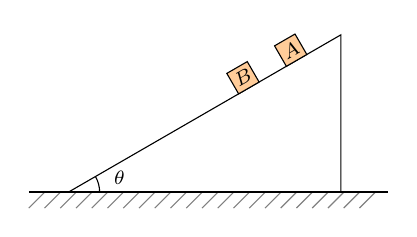
\begin{tikzpicture}[font=\scriptsize]
	\def\TheTa{30}%旋转角度
	\def\LenGth{4}%斜面长度
	\pgfmathsetmacro\CosLenGth{\LenGth*cos(\TheTa)+.4}
	\begin{scope}[rotate=\TheTa]	
		\draw (0,0)--++(\LenGth,0)--++(-120:2);
        \draw[fill=orange!40] (2.5,0) rectangle(2.8,.3)node[midway,rotate=30]{\(B\)} (3.2,0) rectangle(3.5,.3)node[midway,rotate=30]{\(A\)};
	\end{scope}
	\draw (.4,0) arc(0:\TheTa:.4);
	\node at(.65,.18){\(\theta\)};
	\foreach \x in{-.5,-.3,...,\CosLenGth}
		\draw[gray] (\x,-.2)--++(.2,.2);
	\draw[thick] (-.5,0)--({\CosLenGth+.2},0);
\end{tikzpicture}
\begin{answer}
    （1）\(v_{A1} = \frac{4}{9}\) \,\qty{}{m/s}\quad \(v_{B1} = \frac{16}{9}\) \,\qty{}{m/s}（2）0（3）\(\frac{32}{45}(1 - \frac{1}{9^n})\) \,\qty{}{m}

    注意\(\mu_1 = \frac{\sqrt{3}}{3} \)，碰撞后\(A\)做匀速直线运动，\(B\)做匀减速运动，加速度\(a = g(\mu_2\cos\theta - \sin\theta) =\) \,\qty{2.5}{m/s^2}。

    第一次碰撞后\(v_{A1} = \frac{m_1 - m_2}{m_1 + m_2}v_0 = \frac{1}{3}v_0\)\quad \(v_{B1} = \frac{2m_1v_0}{m_1 + m_2} = \frac{4}{3}v_0\)

    第二次碰撞后\(v_{A2} = \frac{1}{3}v_{A1} = \frac{1}{3^2}v_0\)\quad \(v_{B2}= \frac{4}{3}v_{A1} = \frac{4}{3^2}v_0\)

    第\(n\) 次碰撞后\(v_{An} = \frac{1}{3^n}v_0\)\quad \(v_{Bn} = \frac{4}{3^n}v_0\)

    \(B\)第\(n\)次碰撞后沿斜面下滑的位移\(x_n = \frac{v_{Bn}^2}{2a} = \frac{16^2}{5 \times 9^{n + 1}}\) \,\qty{}{m}
\end{answer}